\documentclass[a4paper]{article}

\usepackage{fullpage} % Package to use full page
\usepackage{parskip} % Package to tweak paragraph skipping
\usepackage{tikz} % Package for drawing
\usepackage{amsmath}
%\usepackage{mathaccent}
\usepackage{hyperref}
\usepackage{subfigure}
\usepackage[utf8]{inputenc}
\usepackage[cyr]{aeguill}
\usepackage[frenchb]{babel}
\usepackage{graphicx}
\usepackage[]{algorithm2e}
\usepackage{xcolor}
\usepackage[]{float}
\usepackage{tikz}
\usepackage{listings}
\title{Compte Rendu - TP ETI5-IMI \\ \textit{Shaders avancés et Marching Cubes}}
\author{Di Folco Maxime - Girot Charly}
\date{27/10/2017}


\tikzset{my arrow/.style={
  blue!60!black,
  -latex
  }
  }
  

\begin{document}
\maketitle

%% Explication des noramles, Relecture partie 1 (à completer)
%% Toutes les images d'amelirotaion graphique des textures

\section{Parallax Mapping - Donner l'illusion du relief}
\subsection{Utilisation des textures de normales}
Habituellement, nous utilisons des textures \textit{colorées} appliquées directement sur un maillage. Exemple : dessiner un mur de briques comme sur la Fig.\ref{briques}

\begin{figure}[H]
\centering
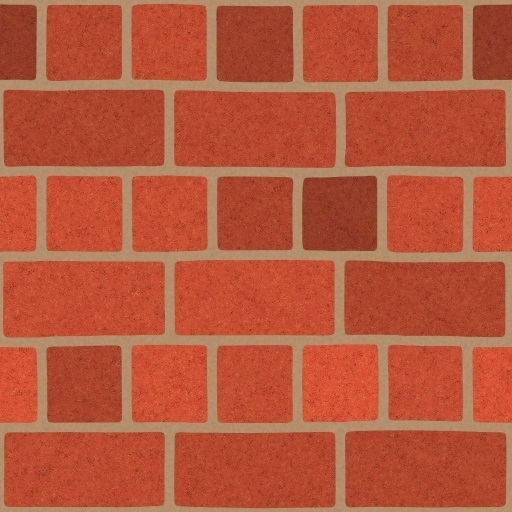
\includegraphics[width=0.3\textwidth]{figures/brick_diffuse.png}
\caption{Texture colorée de briques}
\label{briques}
\end{figure}


Dans ce TP, nous souhaitons utiliser des textures contenant d'autres informations afin de les utiliser pour modifier des caractéristiques de nos images 3D comme les normales sur la Fig.\ref{normales}, ou pour simuler un effet de profondeur comme sur la Fig.\ref{profondeur} dans le but d'avoir un rendu plus réaliste.

\begin{figure}[H]
\centering
\subfigure[]{\label{normales} 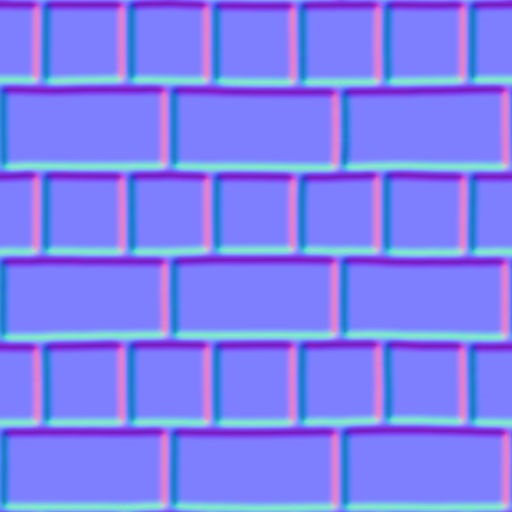
\includegraphics[width=0.3\textwidth]{figures/brick_normales.png}}
\subfigure[]{\label{profondeur} 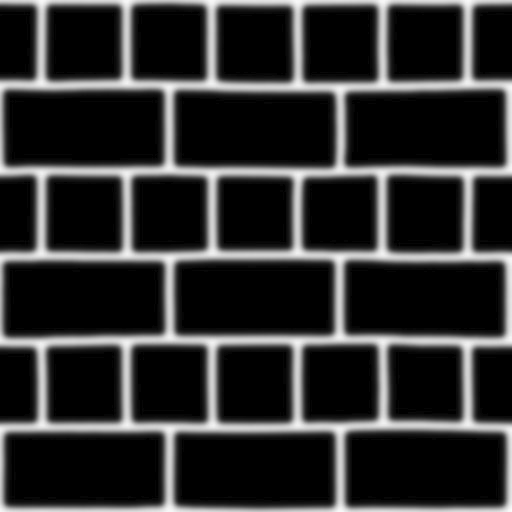
\includegraphics[width=0.3\textwidth]{figures/brick_profondeur.png}}
\caption{Textures contenant les informations de normales (a) et de profondeur (b)}
\end{figure}


Dans un premier temps, on nous fournit un programme qui implémente le normal mapping, dont le résultat est présenté Fig.\ref{NormalesResult}. Cette méthode permet de simuler graphiquement des détails géométriques sur les surfaces représentées. En effet, dans cette méthode, les normales ne sont plus seulement orientées selon l'axe principal $z$ de la surface mais sont désormais liées aux axes $x$,$y$ et $z$ de la surface en fonction de la carte des normales représentée Fig.\ref{normales} où la composante rouge indique une orientation de la normale modifiée selon l'axe $x$, verte pour l'axe $y$ et bleue pour l'axe $z$. Les normales ne sont ainsi plus toutes orientées dans le même sens selon la surface de l'objet, mais orientées différemment selon chaque fragment constituant notre objet comme schématisé Fig.\ref{normalFrag}. On obtient ainsi grâce aux nouvelles orientations de normales, des surfaces contenant plus de détails et donc une impression de relief et un réalisme supérieure comparée à la Fig.\ref{noNormalesResult}.


\begin{figure}[H]
\centering
\subfigure[]{\label{noNormalesResult} 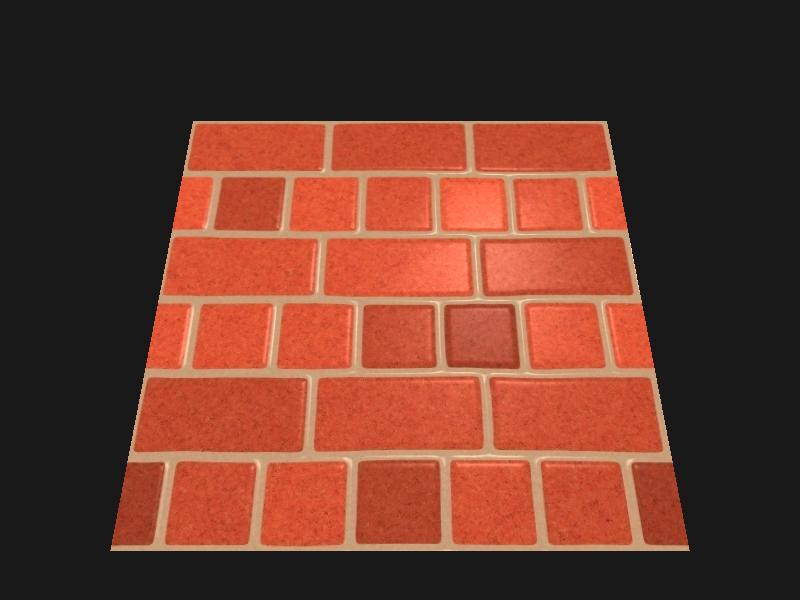
\includegraphics[width=0.3\textwidth]{figures/noNormalMapping.png}}
\subfigure[]{\label{NormalesResult} 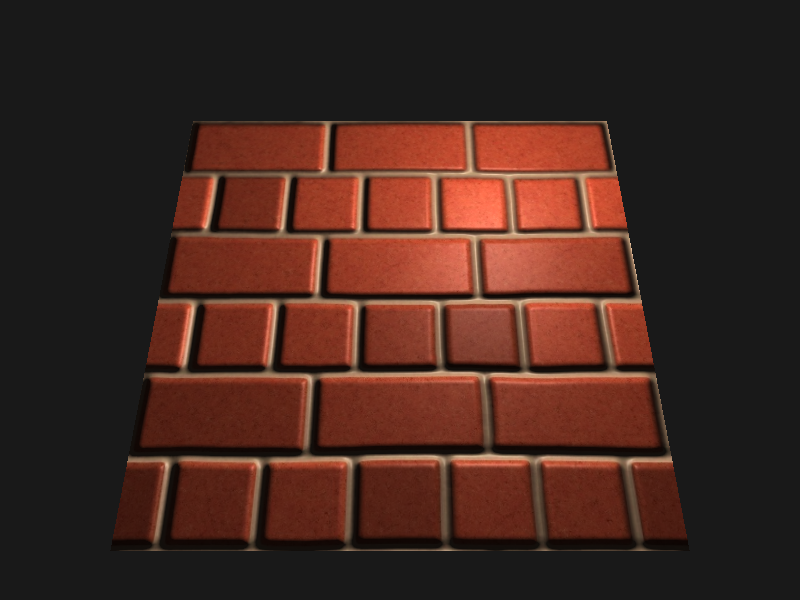
\includegraphics[width=0.3\textwidth]{figures/normalMapping.png}}
\caption{Résultat de l'application de texture couleur (a) auquel on applique la gestion des normales (b)}
\end{figure}

\begin{figure}[H]
\centering
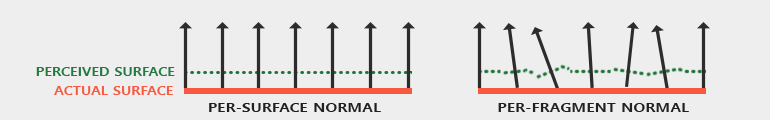
\includegraphics[width=0.5\textwidth]{figures/normalsOrientation.png}
\caption{Principe de l'orientation des normales en parallax mapping - tiré de :  https://learnopengl.com/\#!Advanced-Lighting/Normal-Mapping}
\label{normalFrag}
\end{figure}



Lors de l'application d'un normal mapping avec une carte des normales qui possède majoritairement des normales selon un axe, il faut que la normale interpolée de la surface soit de même direction. Si tel n'est pas le cas, on se retrouve alors avec un problème d'illumination  comme le montre la Fig.\ref{lighting_problem}. En effet les normales ont étés calculés pour chaque fragment selon la carte des textures et non pas selon l'orientation de la normale surfacique. \\

Pour résoudre ce problème d'illumination selon les normales, on se place dans l'espace TBN (Tangente, Bitangente, Normale) de chaque triangle. Dans cet espace, les normales y sont calculés dans ce qui se trouve être un espace local pour chaque triangle. Les normales calculées et modifiées par la carte des hauteurs pointent alors toutes approximativement dans la direction z de chaque triangle peut importe l'orientation finale de l'objet. Il est alors possible de transformer les normales depuis l'espace local tangent vers l'orientation finale de la surface. 


\begin{figure}[H]
\centering
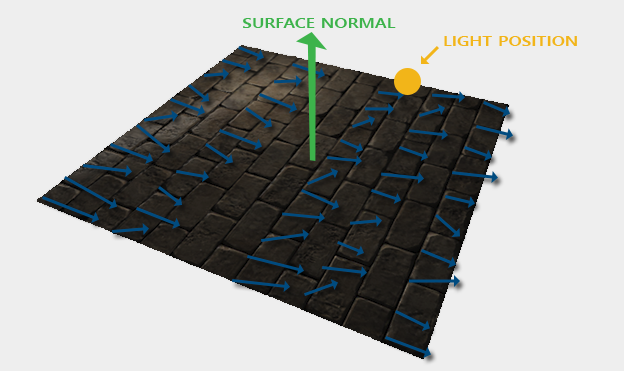
\includegraphics[width=0.5\textwidth]{figures/lighting_problem.png}
\caption{Problème d'orientation des normales pour l'éclairage lors d'un normal mapping classique - tiré de :  https://learnopengl.com/\#!Advanced-Lighting/Normal-Mapping}\label{lighting_problem}
\end{figure}


Pour pouvoir utiliser la méthode de normal mapping, puis ensuite la méthode de parallax que nous allons détailler par la suite, il faut utiliser de nombreuses variables  pour pouvoir calculer la matrice TBN et ensuite calculer les directions de la vue et de la lumière dans nos shaders.
Dans le Vertex Shader nous avons besoin des : \\
- sommets habituels : in vec3 position \\
- données des normales : in vec3 normal \\
- coordonnées de textures : in vec2 $tex_coords$b\\
- tangeantes et bitangeantes calculés precedemment : in vec3 tangent; in vec3 bitangent
 \\

On calcule  alors la matrice TBN pour passer de l'espace local tangent vers l'orientation finale de la surface, avec les lignes de codes suivantes :\\ 
out vec3 $vf\_frag\_pos$ = model * position ;\\
out vec2 $vf\_tex_coords$;\\
out vec3 $vf\_tangent\_light\_pos$ = TBN * $light\_pos$;\\
out vec3 $vf\_tangent\_view\_pos$ = TBN * $view\_pos$;\\
out vec3 $vf\_tangent\_frag\_pos$ = TBN * $vf\_frag_pos$;\\




\subsection{Ajout d'un effet de profondeur avec l'utilisation des cartes de hauteur}
Le normal mapping nous a permis d'obtenir un niveau de détails supplémentaire sur nos textures. Avec peu de données supplémentaires, il est possible de donner une véritable impression de relief en réalisant un Parallax Mapping. Pour cela nous allons utiliser une carte de hauteur afin de modifier par projection les coordonnées de textures à afficher. On utilisera donc dans les shaders une variable supplémentaire $height\_tex$ afin de connaître l'élévation correspondante à chaque coordonnées de textures.Cette méthode simule une impression de relief. \\

Supposons que nous sommes à une position $view\_pos$ et regardons vers la position A comme indiqué Fig.\ref{parallaxtheory}. Le point réel observé ne devrait pas être A correspondant à la coordonnée de texture de départ mais le point B. Il faut alors calculer le point B par projection, ce qui s’avérerait trop complexe. Pour simplifier le problème on cherche alors la position du point P par calcul de l'offset entre le point A  et la projection approximative du point B sur la surface en utilisant la hauteur au point A. Le résultat de cette méthode est présenté Fig.\ref{ParallaxResult}.


\begin{figure}[H]
\centering
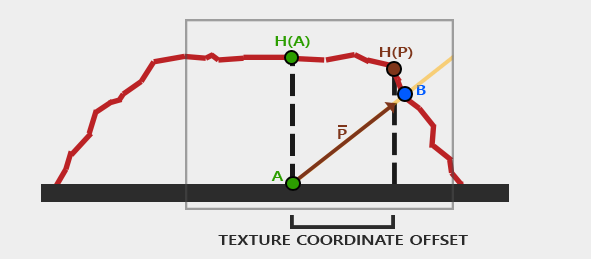
\includegraphics[width=0.8\textwidth]{figures/parala.png}
\caption{Theorie de projection du parallax mapping}
\label{parallaxtheory}
\end{figure}




\begin{figure}[H]
\centering
\subfigure[]{\label{normalResult} 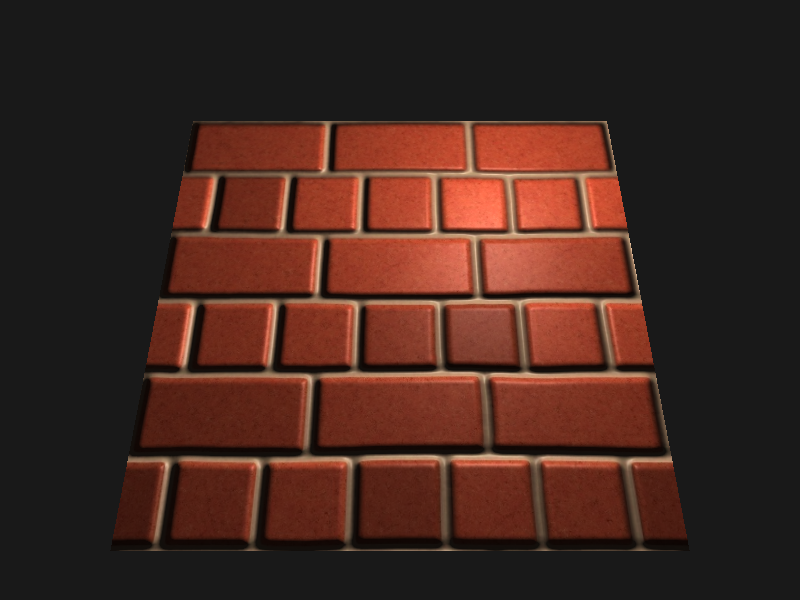
\includegraphics[width=0.3\textwidth]{figures/normalMapping.png}}
\subfigure[]{\label{ParallaxResult} 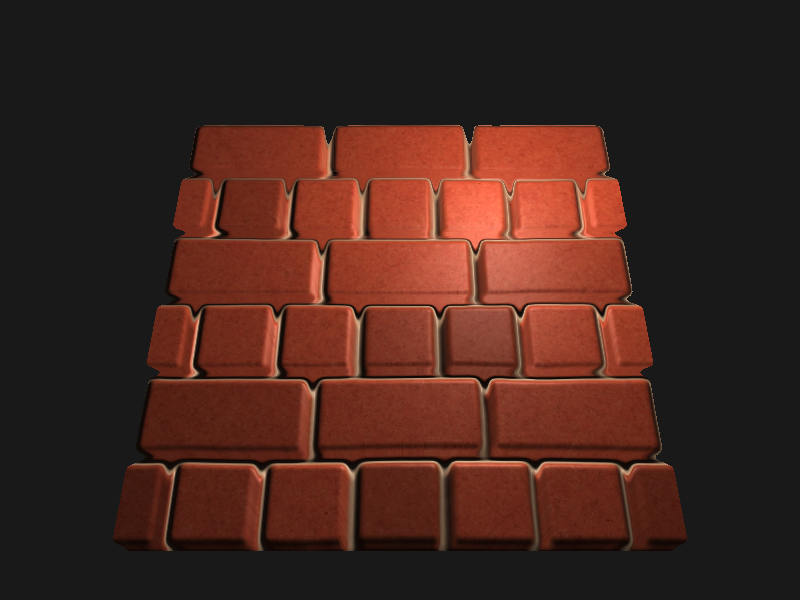
\includegraphics[width=0.3\textwidth]{figures/parallax1.png}}
\caption{Comparaison de la gestion des normales (a) auquel on applique une carte de hauteur (b)}
\end{figure}

Néanmoins, lors du calcul de nos hauteurs nous utilisons un facteur qui permet d'augmenter ou diminuer les hauteurs des coordonnées de nos textures. Si ce facteur est trop petit ou trop grand le rendu ne parait plus réaliste. En effet, l'offset entre les coordonnées de texture réels et les modifiées devient trop important. La surface supérieure des briques semble alors se séparer du mur, ce qui provoque une perte complète du réalisme de la scène.

\begin{figure}[H]
\centering
\subfigure[]{\label{ParallaxResult1} 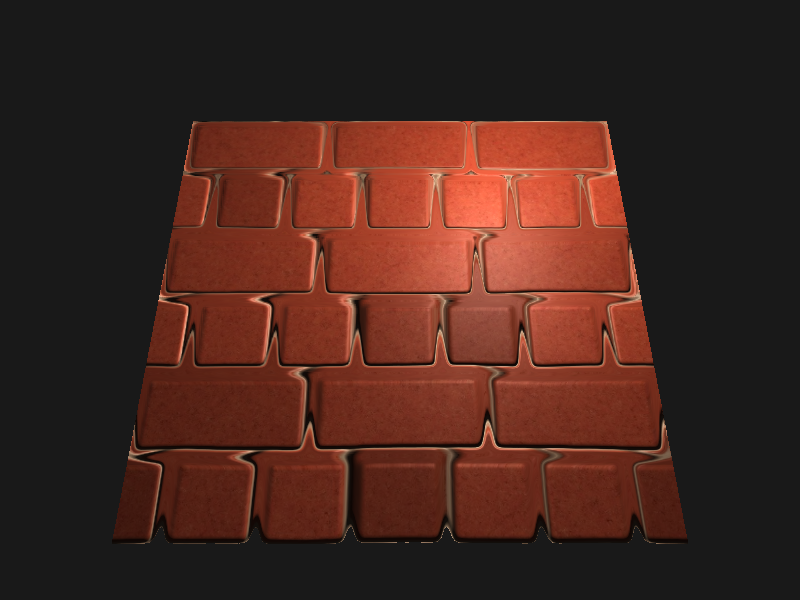
\includegraphics[width=0.3\textwidth]{figures/parallax2.png}}
\subfigure[]{\label{ParallaxResult2} 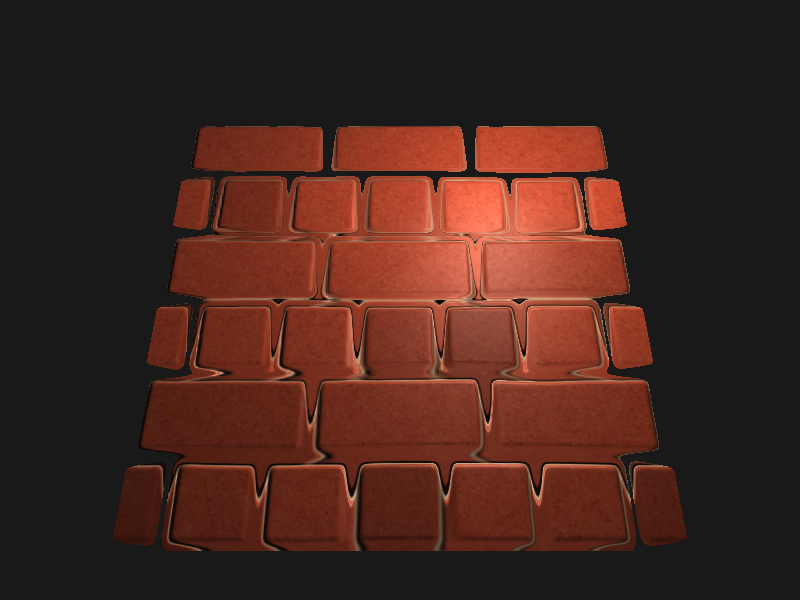
\includegraphics[width=0.3\textwidth]{figures/parallax3.png}}
\caption{Résultats de la carte des profondeurs pour un facteur de hauteur trop faible (a) trop haut (b)}
\end{figure}


\section{Marching Cubes}

\subsection{Présentation Générale}

L'algorithme des \textit{marchings cubes} à pour but d'extraire des meshs à partir d'un ensemble de points de l'espace, définit comme un champ scalaire ou à chacun des points 3D est associé sa densité. Une valeur positive de densité correspond à un point de la surface solide et une valeur négative à un espace vide. Grâce au GPU, l'espace est subdiviser en 3*3*8 blocs de 48*48*48 blocs élementaires (voxels) reprensentés par des cubes. C'est au sein de chacun des cubes que l'algorithme remplace et il faut alors distinguer 256 ($2^8$ : 8 angles pour le cube) cas différents : 
\begin{itemize}
\item Cas 0 : Les 8 angles du cube sont de densité négative : le cube est complètement en dehors de la surface => Rien à dessiner.
\item Cas $ 1 \to 254$ : Au moins un des 8 angles n'est pas de même signe que les autres : On cherche alors au sein d'une table de correspondance pour savoir combien de polygones seront générées au sein du cube et comment les construire. La Fig.\ref{marchingCubes} présente les principaux cas possibles parmi les 256 possibles. 
\item Cas 255 : Les 8 angles du cube sont de densité positive : le cube est completement à l'intérieur de la surface => Rien à dessiner puisqu'on ne represente graphiquement que les bordures d'une surface. 

\end{itemize}

\begin{figure}[H]
\centering
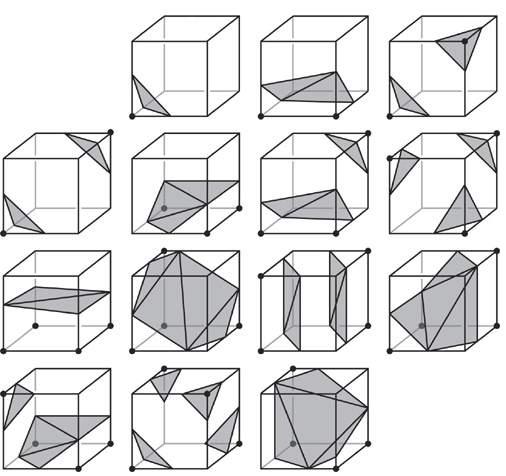
\includegraphics[width=0.5\textwidth]{figures/marchingCubes.png}
\caption{Illustration des principaux cas possibles pour la representation des polygones avec l'algorithme des marchings cubes}
\label{marchingCubes}
\end{figure}

La Fig.\ref{pipeline} montre l’enchaînement des différents shaders pour la réalisation des marchings cubes.

\begin{figure}[H]
\centering
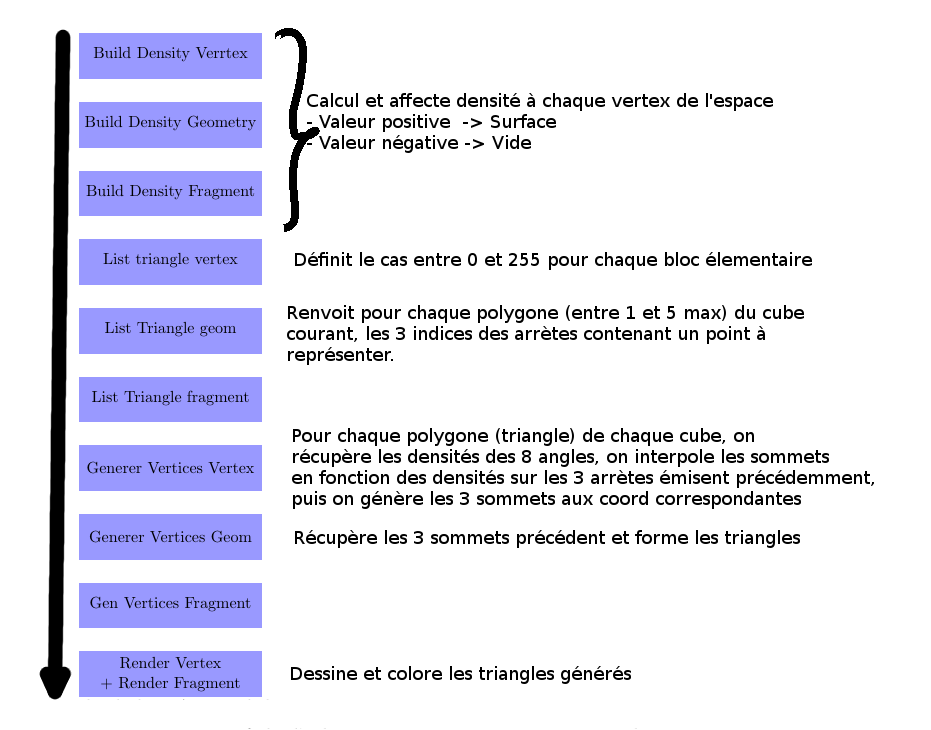
\includegraphics[width=0.7\textwidth]{figures/pipeline3.png}
\caption{Pipeline pour la réalisation de l'algorithme marching cubes avec explications des blocs principaux}
\label{pipeline}
\end{figure}
%
%\begin{center}
%\begin{tikzpicture}
%
%
%\draw[step=0.5cm,white,very thin] (-6,-5) grid (6,10) ;
%\fill[blue!40!white] (-2,10) rectangle (2,9);
%\node[above] at (0,9.25){Build Density Verrtex};
%
%
%
%\fill[blue!40!white] (-2,8.5) rectangle (2,7.5) ;
%\node[above] at (0,7.75){Build Density Geometry };
%
%\fill[blue!40!white] (-2,7) rectangle (2,6);
%\node[above] at (0,6.25){Build Density Fragment };
%
%
%\fill[blue!40!white] (-2,5.5) rectangle (2,4.5);
%\node[above] at (0,4.75){List triangle vertex };
%
%\fill[blue!40!white] (-2,4) rectangle (2,3);
%\node[above] at (0,3.25){List Triangle geom};
%
%\fill[blue!40!white] (-2,2.5) rectangle (2,1.5);
%\node[above] at (0,1.75){List Triangle fragment };
%
%\fill[blue!40!white] (-2,1) rectangle (2,0);
%\node[above] at (0,0.25){Generer Vertices Vertex };
%
%\fill[blue!40!white] (-2,-0.5) rectangle (2,-1.5);
%\node[above] at (0,-1.25){Generer Vertices Geom};
%
%\fill[blue!40!white] (-2,-2) rectangle (2,-3);
%\node[above] at (0,-2.75){Gen Vertices Fragment };
%
%\fill[blue!40!white] (-2,-3.5) rectangle (2,-4.5);
%\node[above] at (0,-4){Render Vertex  };
%\node[above] at (0,-4.5){+ Render Fragment};
%
%
%\node[above] at (0,-5){Ordre d'utilisation des shaders - Ajouter Fleches et explications };
%\end{tikzpicture}
%\end{center}


\subsection{Amélioration de l'algorithme}

Jusqu'a présent le calcul de normales pour chaque triangle était constant (chaque polygone possède la même normale). On choisit alors d'intérpoler  les normales pour chaque triangle en fonction du gradient de la fonction de densité en chaque point, le résultat est présenté Fig.\ref{mcNormalResult}. 

\begin{lstlisting}[language=C++,
                   directivestyle={\color{black}}
                   emph={int,char,double,float,unsigned},
                   emphstyle={\color{blue}}
                  ]]
// pos : position du voxel courant
vec3 calc_normal(vec3 pos)
{
  vec3 grad = vec3(1.);   // Ancienne normale 
  float d = 1.0/48.0;     // Ecart entre deux fragments pour calcul du gradient
  // Calcul du gradient dans les 3 directions x,y,z
  grad.x = text_density( pos + vec3( d, .0, .0)) - text_density( pos+ vec3(-d, .0, .0));
  grad.y = text_density( pos + vec3( .0, d, .0)) - text_density( pos+ vec3( .0,-d, .0));
  grad.z = text_density( pos + vec3( .0, .0, d)) - text_density( pos+ vec3( .0, .0,-d));
  return normalize(grad);
}
\end{lstlisting}

On cherche encore a amélioré le résultat en interpolant correctement les sommets des points sur chaque arrête. En effet ils étaient précédemment toujours calculés au milieu des arrêtes du cube sans tenir compte de la densité de chaque sommet, ce qui à pour effet de rendre une sphère avec un aspect crénelé. On choisit alors d'interpoler linéairement et le résultat est présenté Fig.\ref{mcInterResult} : 
\begin{lstlisting}[language=C++,
                   directivestyle={\color{black}}
                   emph={int,char,double,float,unsigned},
                   emphstyle={\color{blue}}]]
// v0, v1 : positions des sommets
// l0, l1 : densite des sommets v0 et v1
vec3 vertexInterp(vec3 v0, float l0, vec3 v1, float l1)
{
  // return (v0 + v1) / 2; // Ancienne interpolation
  return (l1*v0 - l0*v1)/(l1-l0); // Interpolation lineaire
}
\end{lstlisting}



\begin{figure}[H]
\centering
\subfigure[]{\label{mc0} 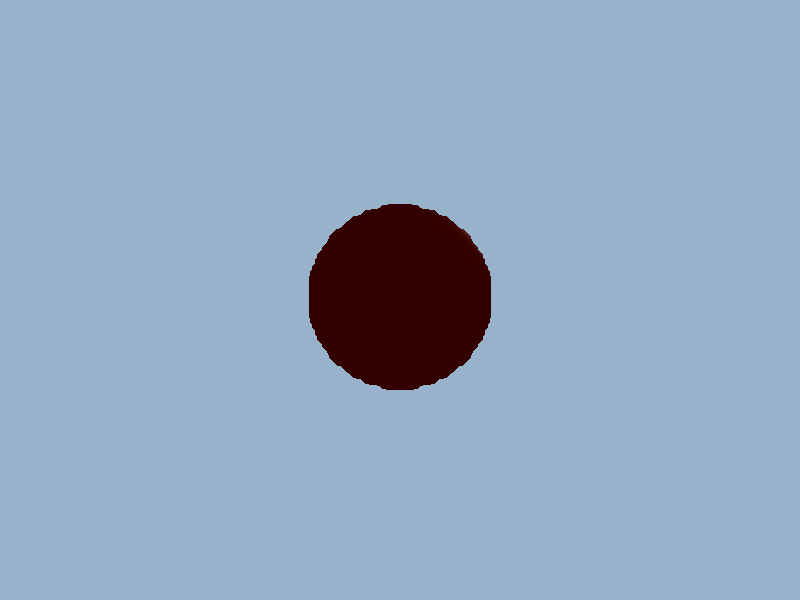
\includegraphics[width=0.3\textwidth]{figures/mc0.png}}
\subfigure[]{\label{mcNormalResult} 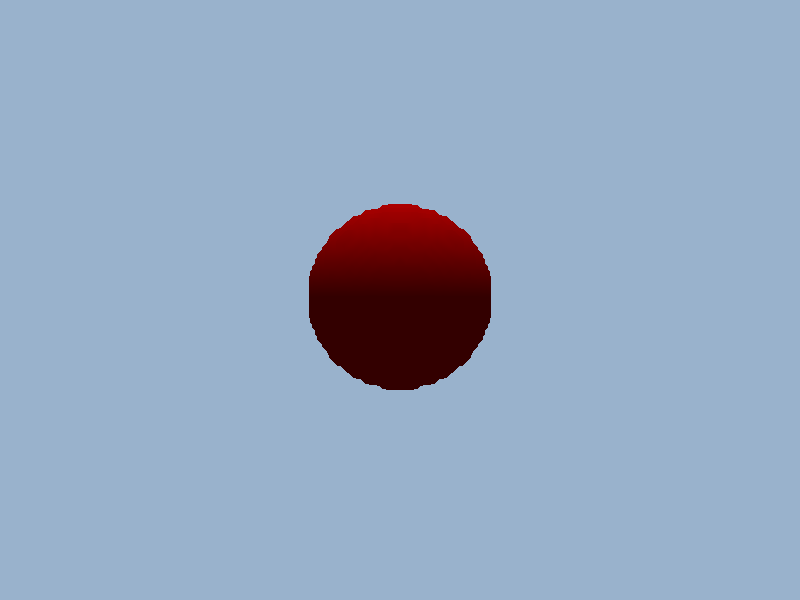
\includegraphics[width=0.3\textwidth]{figures/mcnorm.png}}
\subfigure[]{\label{mcInterResult} 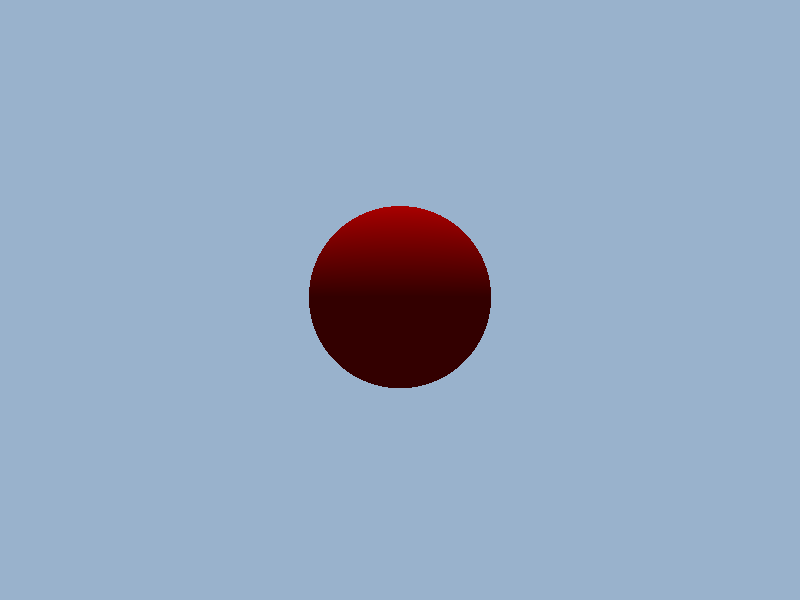
\includegraphics[width=0.3\textwidth]{figures/mcnorminterp.png}}
\caption{Marching Cubes Original (a) ; Calcul des normales fonction du gradient de la fonction de densité (b); Interpolation linéaire de placement des vertex par rapport aux arrètes (c)}
\end{figure}


\subsection{Fonction de densité}

Avec le nouveau calcul des normales et les interpolations des sommets corrects, il est désormais intéressant de générer des structures plus chaotique, plus aléatoire, plus intéressantes. On s'inspire alors de l'algorithme de calcul de la densité présenté par NVidia : "Cascades par Ryan Geiss et Michael Thompson". On présente nos différents résultat de fonctions de densité tout d'abord pour des fonctions de densité simple (Sphère, Torus Fig.\ref{sphere} et \ref{torus}) puis par utilisation de l'algorithme NVidia Fig\ref{rock}. On fais également varier certains paramètres de cet algorithme (comme suit) pour obtenir notre résultat final Fig.\ref{rockf} avec ou sans bruit.

\begin{lstlisting}[language=C++,
                   directivestyle={\color{black}}
                   emph={int,char,double,float,unsigned},
                   emphstyle={\color{blue}}]]
                   
/** Return a density function to create a self-shaped rock  */
float density_perso(vec3 ws)
{
    //ws coordinates UV of fragments
     float f = 0; // density function
     
    //Add noise to fragments so the result isn't flat but irregular
     ws.yz   += 0.5*Noise_MQ_unsigned(ws/10,noiseVol0).xy 
	    + 0.5*Noise_MQ_unsigned(ws/10,noiseVol1).xy
	    + 0.5*Noise_MQ_unsigned(ws/10,noiseVol2).xy
	    + 0.3*Noise_MQ_unsigned(ws/10,noiseVol3).xy;
    
    //Create 4 pillar center in a xy plane (NB : xy OpenGL = xz in most of the case)
    vec2 pillar[4];
    pillar[0] = vec2(0.4,-0.8);
    pillar[1] = vec2(0.4,1.0);
    pillar[2] = vec2(-0.8,-0.4);
    pillar[3] = vec2(-0.4,1.0);

    
    for(int k=0; k<4; k++)
    {
      f += 1 / length(ws.xy - pillar[k].xy) -1; // add positive value at pillar
    }
    f -= 1 / length(ws.xy) - 3; //Add negative values going down the center (water flow channel)
    f = f - 2*pow(length(ws.xy), 3); // Add strong negative values at outer edge (Help to keep solid rock in bounds)
    
    //Rotate the values as the slice's Z coord changes. 
    vec2 v = vec2(cos(ws.z),3*sin(ws.z));
    f += dot(v,ws.xy);
    
    //Shelves : periodically add positive values based on slice's Z coord. 
    f += 5*cos(ws.z);
    
    return f;
}
\end{lstlisting}

\begin{figure}[H]
\centering
\subfigure[]{\label{sphere} 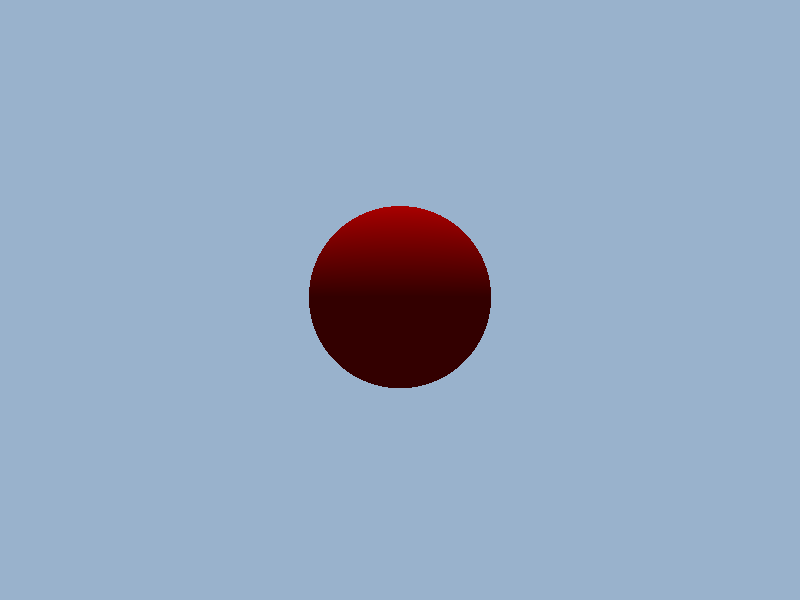
\includegraphics[width=0.3\textwidth]{figures/mcnorminterp.png}}
\subfigure[]{\label{torus} 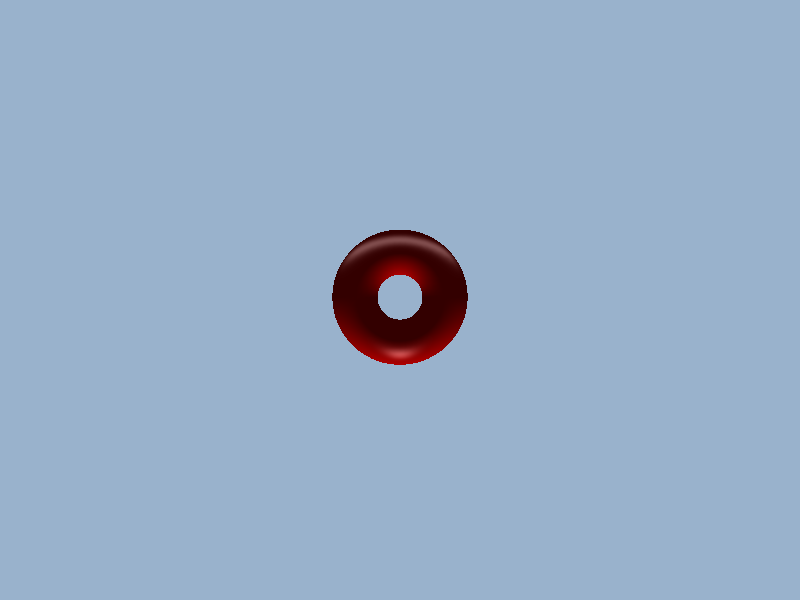
\includegraphics[width=0.3\textwidth]{figures/torus.png}}
\subfigure[]{\label{rock} 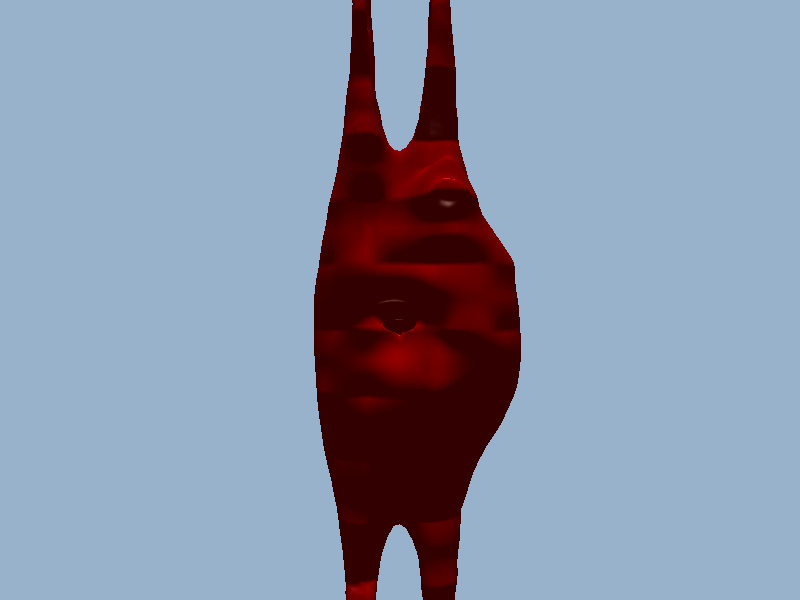
\includegraphics[width=0.3\textwidth]{figures/chelouA.png}}
\caption{Marching Cubes avec différentes fonctions de densite : Boule (a), Torus (b), Création de roches (c)}
\end{figure}
\begin{figure}[H]
\centering
\subfigure[]{\label{rockfnonoise} 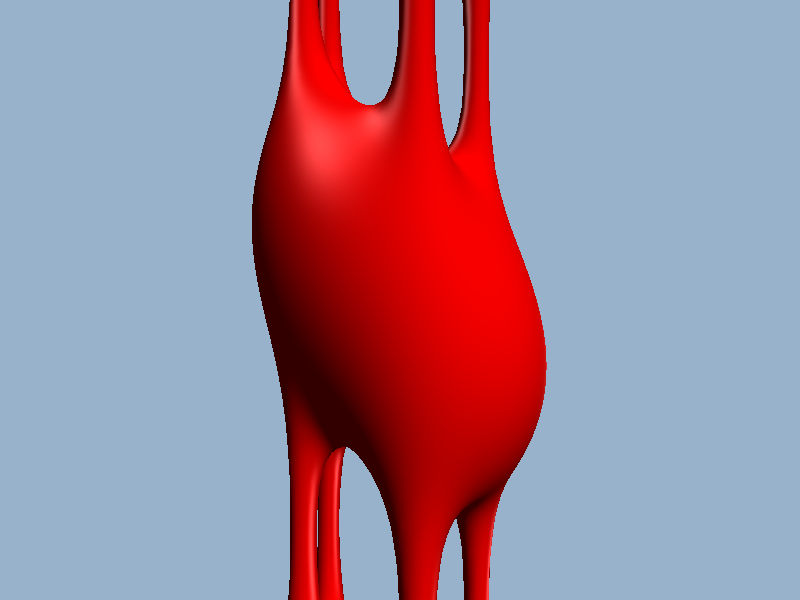
\includegraphics[width=0.3\textwidth]{figures/finalnonoise.png}}
\subfigure[]{\label{rockf} 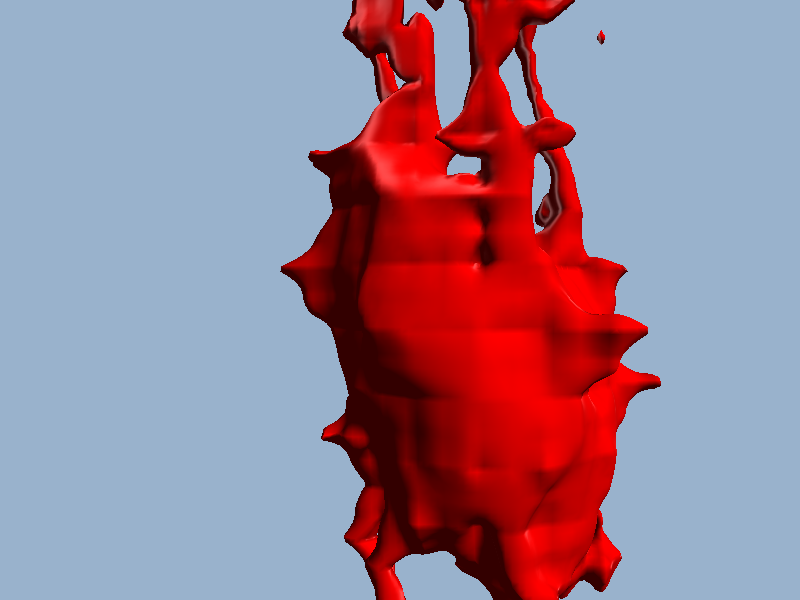
\includegraphics[width=0.3\textwidth]{figures/finalDensity.png}}
\caption{Densité finale retenue non bruitée (a), bruitée (b)}
\end{figure}

\subsection{Amélioration graphique \& Textures}



Le but de cette partie est d'appliquer une texture quelconque à la surface. Or les coordonées de textures n'existe pas et il serait impossible d'en obtenir des cohérentes au préalable étant donné la surface quelconque. Ce sont ainsi les coordonnées spatiales des sommets qui sont utilisées comme coordonnées de textures en ne prenant que deux dimensions sur les 3. Pour ne pas privilégier une seule direction sur laquelle projeté la texture (choisir x et y comme coordonnées de texture reviendrait à projeter la texture selon l'axe z), les deux coordonnées sont choisies par pondération des normales. Les textures sont alors projetés sur l'axe prépondérant et les 2 autres axes sont utilisés comme coordonnées de texture. La Fig.\ref{normalesCouleurs} représente cet affichage avec des couleurs pondérées par les normales : Rouge(x), Vert(y), Bleu(z). 

\begin{figure}[H]
\centering
\subfigure[ ]{\label{normal1} 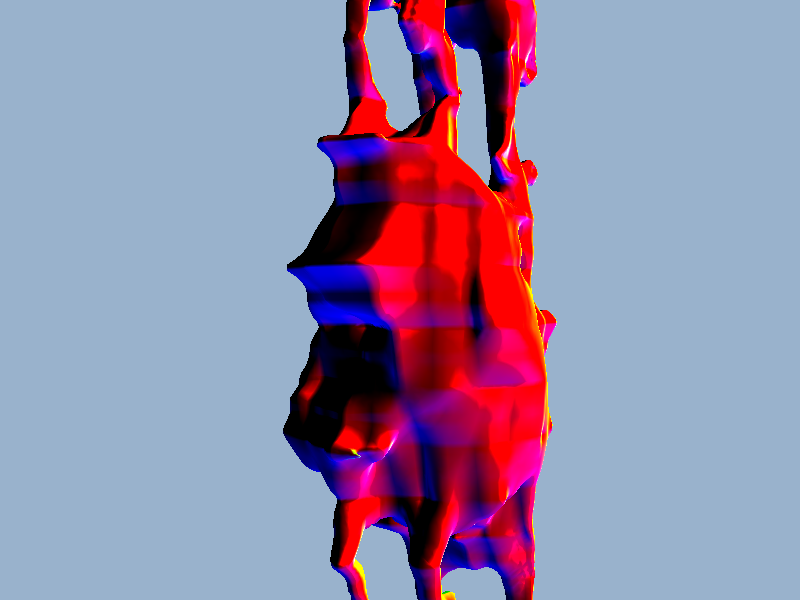
\includegraphics[width=0.3\textwidth]{figures/normales1.png}}
\subfigure[ ]{\label{normal2} 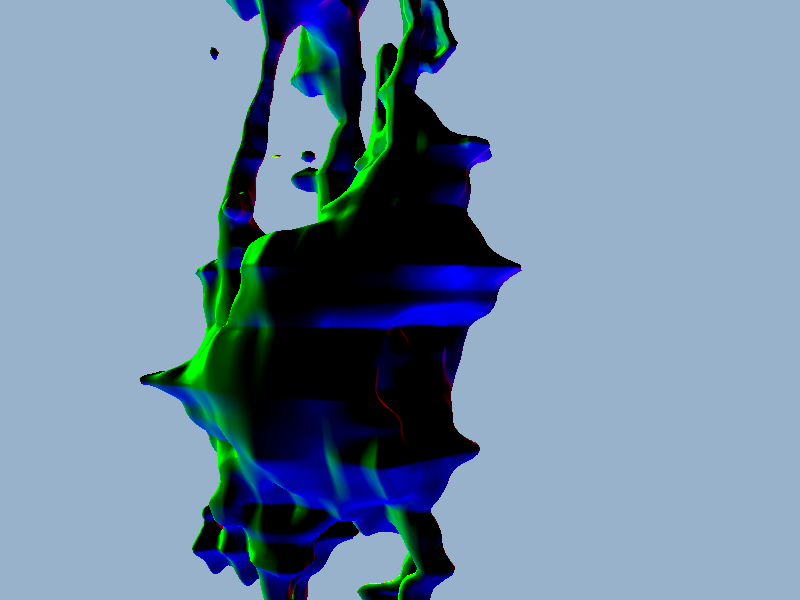
\includegraphics[width=0.3\textwidth]{figures/normales2.png}}
\subfigure[ ]{\label{normal3} 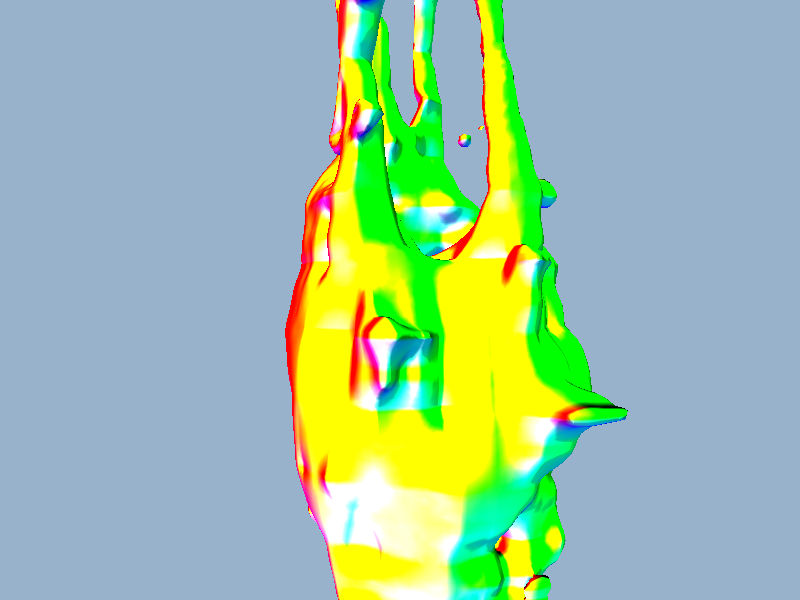
\includegraphics[width=0.3\textwidth]{figures/normales3.png}}
\caption{Application des normales pondérés représentées par le mélange des 3}
\label{normalesCouleurs}
\end{figure}

Enfin, on remplace l'affichage couleurs par l'affichage de textures comme suit : 

La Fig.\ref{normalestextures} présente les résultats pour l'application d'une texture brique et l'application d'une texture rocheuse. 
\begin{figure}[H]
\centering
\subfigure[ ]{\label{normalt1} 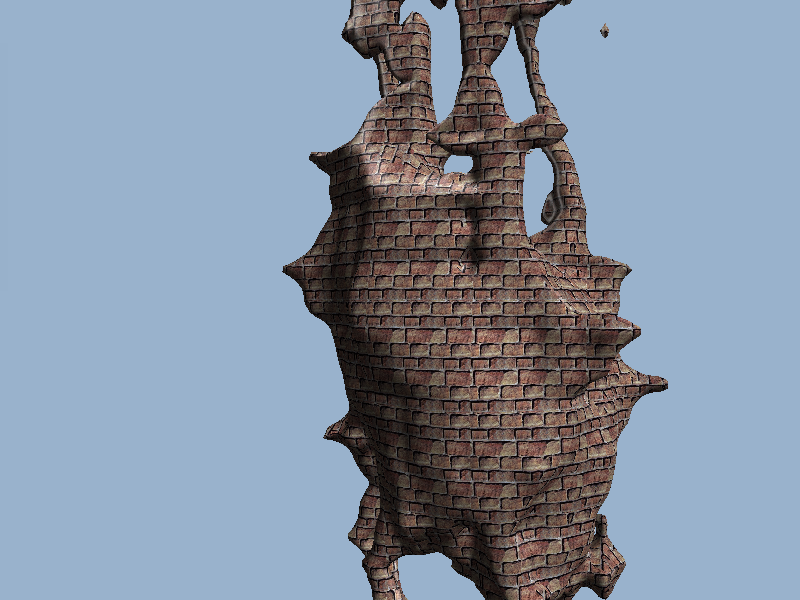
\includegraphics[width=0.45\textwidth]{figures/normalesPondereBrique.png}}
\subfigure[ ]{\label{normalt2} 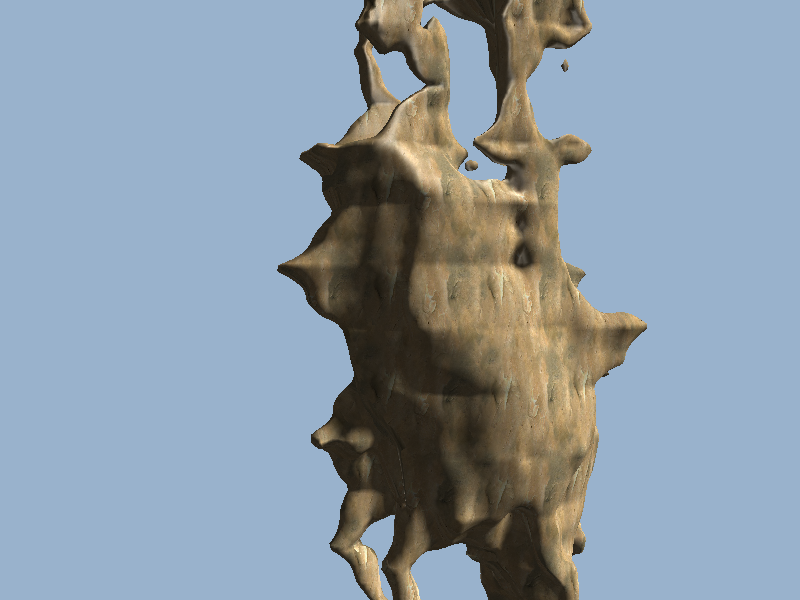
\includegraphics[width=0.45\textwidth]{figures/normalesTextures.png}}
\caption{Application des coordonnées de texture par pondération des normales}
\label{normalestextures}
\end{figure}


Choix de la direction de projection relativement aux normales et définition des coordonées de textures égales aux coordonnées de position : 

\begin{lstlisting}[language=C++,
                   directivestyle={\color{black}}
                   emph={int,char,double,float,unsigned},
                   emphstyle={\color{blue}}]]
vec2 coord_tex;
vec3 test_color;

if(abs(vf_normal.x) > abs(vf_normal.y) && abs(vf_normal.x) > abs(vf_normal.z))
  {
    coord_tex = vf_position.yz;
//     test_color = vec3(1.5*vf_normal.x, vf_normal.y, vf_normal.z);//Ponderation de la couleur selon la direction principale pour un rendu plus naturel
  }
  else if(abs(vf_normal.y) > abs(vf_normal.x) && abs(vf_normal.y) > abs(vf_normal.z))
  {
    coord_tex = vf_position.xz;
//     test_color = vec3(vf_normal.x, 1.5*vf_normal.y, vf_normal.z);//Ponderation de la couleur selon la direction principale pour un rendu plus naturel
  }
  else
  {
    coord_tex = vf_position.xy;
//     test_color = vec3(vf_normal.x, vf_normal.y, 1.5*vf_normal.z); //Ponderation de la couleur selon la direction principale pour un rendu plus naturel
  }
   test_color = 5*vec3(vf_normal.x, vf_normal.y, vf_normal.z); //Couleur melangeant les 3 vues des normales 
                   
\end{lstlisting}

Définition de la couleur d'après les nouvelles normales : 
\begin{lstlisting}[language=C++,
                   directivestyle={\color{black}}
                   emph={int,char,double,float,unsigned},
                   emphstyle={\color{blue}}]]
 
float blend_weights = abs(100)-0.2;
blend_weights *=7;
blend_weights = pow(blend_weights, 3);
blend_weights = max(0,blend_weights);
blend_weights /= dot(blend_weights,1);
  
const float freq = 0.17;
//vec4 texcolor = vec4(1.0,0.,0.,1.0); // Affichage du volume en rouge
//vec4 texcolor = vec4(blend_weights*test_color,1); //Affichage du volume avec couleurs par normales ponderees
vec4 texcolor = texture(blend_weights*myTexture, coord_tex); // Affichage du volume avec texture    
...
color =  occ_light * occ_light * (blended_color * 0.2 + 0.6 * diffuse + 0.3 * vec4(vec3(specular), 1.0));              
\end{lstlisting}

Finalement la dernière étape est l'application de l'occlusion de la lumière permettant de savoir quelle quantité de lumière, en chaque point, reste bloqué dans la texture ou parviennent à la caméra. Cela permet un rendu plus naturelle des ombres comme montré Fig.\ref{finalRendu}.
\begin{figure}[H]
\centering
\label{normalt1} 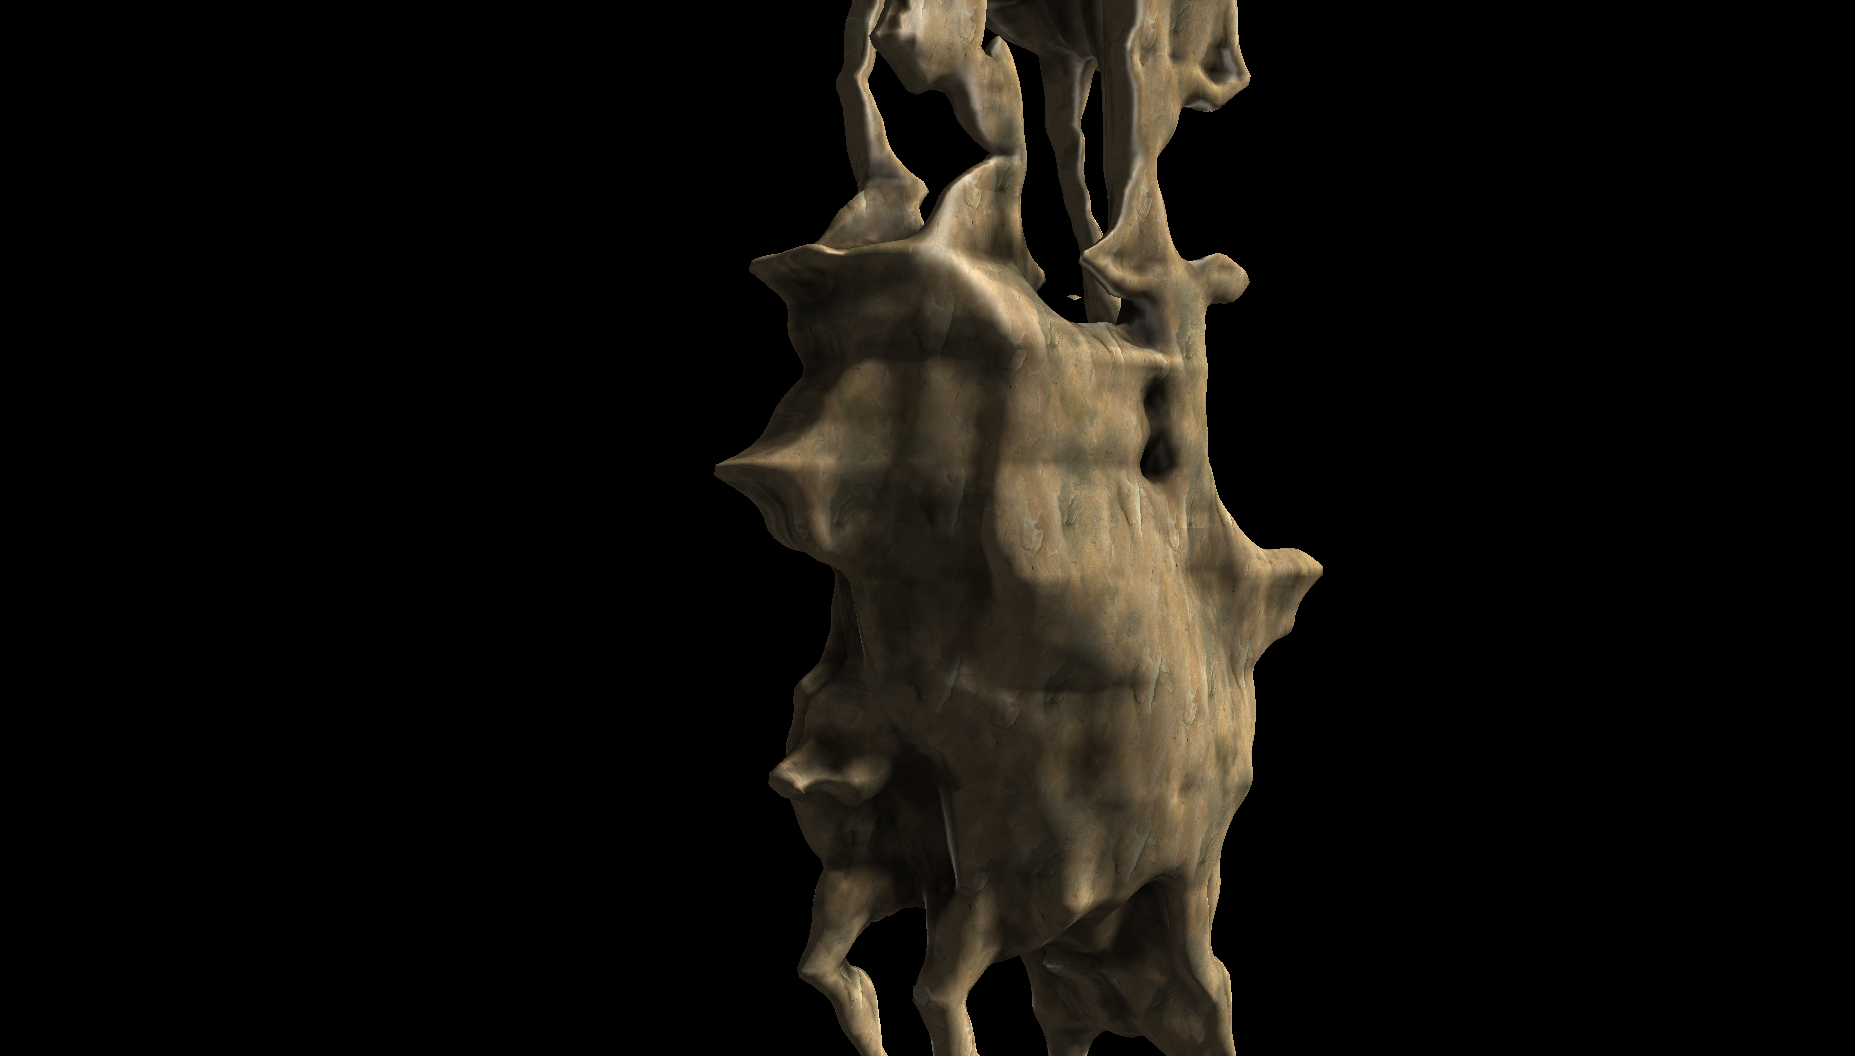
\includegraphics[width=0.9\textwidth]{figures/final.png}
\caption{Occlusion de la lumière et rendu final}
\label{finalRendu}
\end{figure}

\section{Problèmes rencontrés}

- En parallax mapping, il n'a pas été compris pourquoi diviser par la composante z améliore encore les résultats en donnant un relief d’autant plus important que la vue est rasante
- Nous avons également rencontré des difficultés lors de la tentative d'implémentation du parallax mapping + Marching Cubes qui aurait été intéressante sur le rendu final en raison de la forme de notre volume final. En effet nous n'avons pas réussi à savoir ou placer les informations de parallax (créer un render.geom et utiliser un TF pour calculer les Tangeantes Bitangeants pour chaque triangle ? ). Il serait intéressant à titre personnel de comprendre comment faire cette combinaison.

\bibliographystyle{plain}
\bibliography{bibliography.bib}
\end{document}